\section{Anexo}

\subsection{Introduccion (reentrega)}

...

Dicho esto, empezamos a plantear posibles soluciones para el problema. Lo primero que se nos vino a la mente es la idea de hacer uso de algún tipo de ordenamiento, ya sea ordenando por los tiempos de Scaloni o los ayudantes, en relación a cuánto tardaría cada uno. Lo que nos ayudó a volcarnos por el lado de ordenar por los tiempos de los ayudantes fue el siguiente:

\begin{itemize}
    \item El tiempo total que tarda Scaloni siempre va a ser el mismo, no importa cómo ordenemos los videos a ver. Sea $s_i$ el tiempo que tarda Scaloni para analizar el rival $r_i$ y haciendo uso de la propiedad conmutativa de la suma se demuestra:
    	\begin{center}
        	\[ \sum_{i=1}^{n} s_i = s_1 + s_2 + ... + s_n = s_n + s_{n-1} + s_{n-2} + ... + s_1 = \sum_{i=1}^{n} s_i \]
    	\end{center}
    
    \item Por más que Scaloni termine de ver el último video del último rival, va a quedar que después un ayudante analice el video, por lo que es más importante el tiempo que va a tardar este último ayudante que el que va a tardar Scaloni.
\end{itemize}

Ahora bien, ya tenemos definido por donde queremos encarar el problema, pero todavía falta definir en qué orden queremos que los videos se visualicen dependiendo de los ayudantes, si los más rápidos primero o viceversa. Acá entra en juego un factor muy importante a tener en cuenta: \textbf{los ayudantes analizan los videos inmediatamente termina Scaloni de ver el video, y el análisis de cada ayudante es independiente a los otros}. Esto quiere decir que si Scaloni termina un video, inmediatamente uno de los ayudantes se pondrá a analizarlo. Y si Scaloni termina otro video, otro ayudante podrá empezar a analizar ese video, no importa si el anterior terminó de realizar su análisis o no. Esto nos ha llevado a tomar la decisión de ordenar por el tiempo de los ayudantes del que más tarde al que menos, por los siguientes puntos:

\begin{itemize}
    \item Los ayudantes pueden analizar un video independientemente de si el anterior haya terminado o no su análisis.
    \item Sea $t_i$ el tiempo total tomado para analizar al rival $r_i$, $s_i$ el tiempo que tarda Scaloni y $a_i$ el tiempo que tarda el ayudante en analizar ese video:
    	\begin{center}
        	\[ \sum_{i=1}^{n} t_i = \sum_{i=1}^{n} s_i + a_i = s_1 + a_1 + s_2 + a_2 + ... + s_n + a_n \]
    	\end{center}
	Suponiendo por ejemplo que el análisis hecho por $a_n$ es el que más tarda, y teniendo en cuenta que cada ayudante es independiente al resto, el tiempo total para analizar todos los videos va a ser
    	\begin{center}
        	\[ t_{total} = t_{scaloni} + a_n \]
    	\end{center}
	donde $t_{scaloni}$ es el tiempo total de Scaloni en analizar todos los rivales. Entonces si el ayudante $a_n$ es el que más tarda, el tiempo no será el óptimo sino todo lo contrario, será el peor de todos ya que el que más tarda es el último en empezar a analizar a su correspondiente rival.
    \item Por ese motivo, conviene que los ayudantes que más tarden estén al principio, ya que tienen tiempo hasta que Scaloni termine todos los videos para terminar. Y los ayudantes que menos tardan, estarán al final, de modo que si Scaloni termina, los que les falten sabemos que son los más rápidos y terminan lo antes posible, acortando el valor de $a_n$.
\end{itemize}


\subsection{Algoritmo para encontrar el tiempo óptimo (reentrega)}

...\footnote{Aclaración: se ha suprimido el código donde se obtenían los datos en la parte del informe original.}

La complejidad del algoritmo para ordenar todos los datos es $\mathcal{O}\left(n \log n\right)$, ya que el método \textit{sort} de Python tiene esa complejidad (\href{https://www.geeksforgeeks.org/sort-in-python/}{complejidad del método \textit{sort}}) y la función auxiliar que usa como \textit{key} para ordenar es $\mathcal{O}(1)$. Luego, recorrer todo los datos ya ordenados e ir procesando la información es $\mathcal{O}(n)$, ya que solo recorre el arreglo y va sumando los valores correspondientes a las variables declaradas en $\mathcal{O}(1)$. Por lo tanto, la complejidad final del algoritmo propuesto es $\mathcal{O}\left(n \log n\right)$.

...

\subsection{Mediciones (reentrega)}

Se realizaron mediciones en base a crear pruebas de distintos tamaños y tomar su tiempo de ejecución individualmente, y en base a los datos recolectados hacer el gráfico. Los datos fueron desde 100.000 hasta 1.000.000 elementos, los cuales los tiempos tanto de Scaloni como los ayudantes para cada uno de los rivales fue un número aleatorio desde 1.000 hasta 100.000.

\begin{figure}[H]
    \centering
    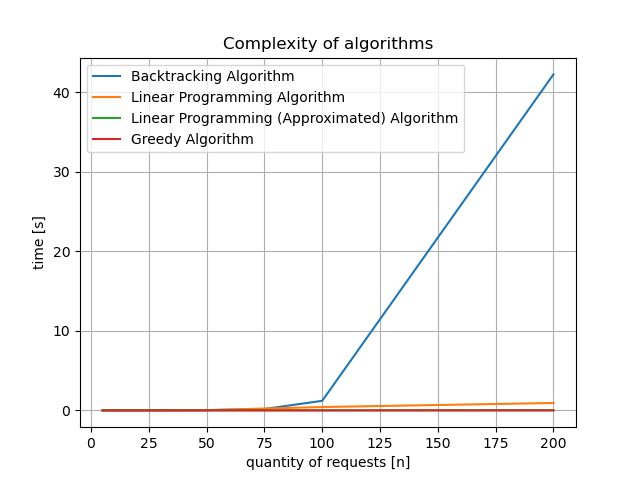
\includegraphics[width=1\textwidth]{img/graphic.png}
\end{figure}

Como se puede apreciar, la complejidad del algoritmo se asemeja a la de $\mathcal{O}\left(n \log n\right)$, bien como se analizó anteriormente. El hecho de que varíe la pendiente de las funciones no se debe dar mucha importancia, sino que lo importante es que en términos de "linealidad" ambas se asemejan.

Por otro lado, se han hecho mediciones de otros algoritmos para poder comparar con el propuesto por nosotros:

\begin{figure}[H]
	\centering
	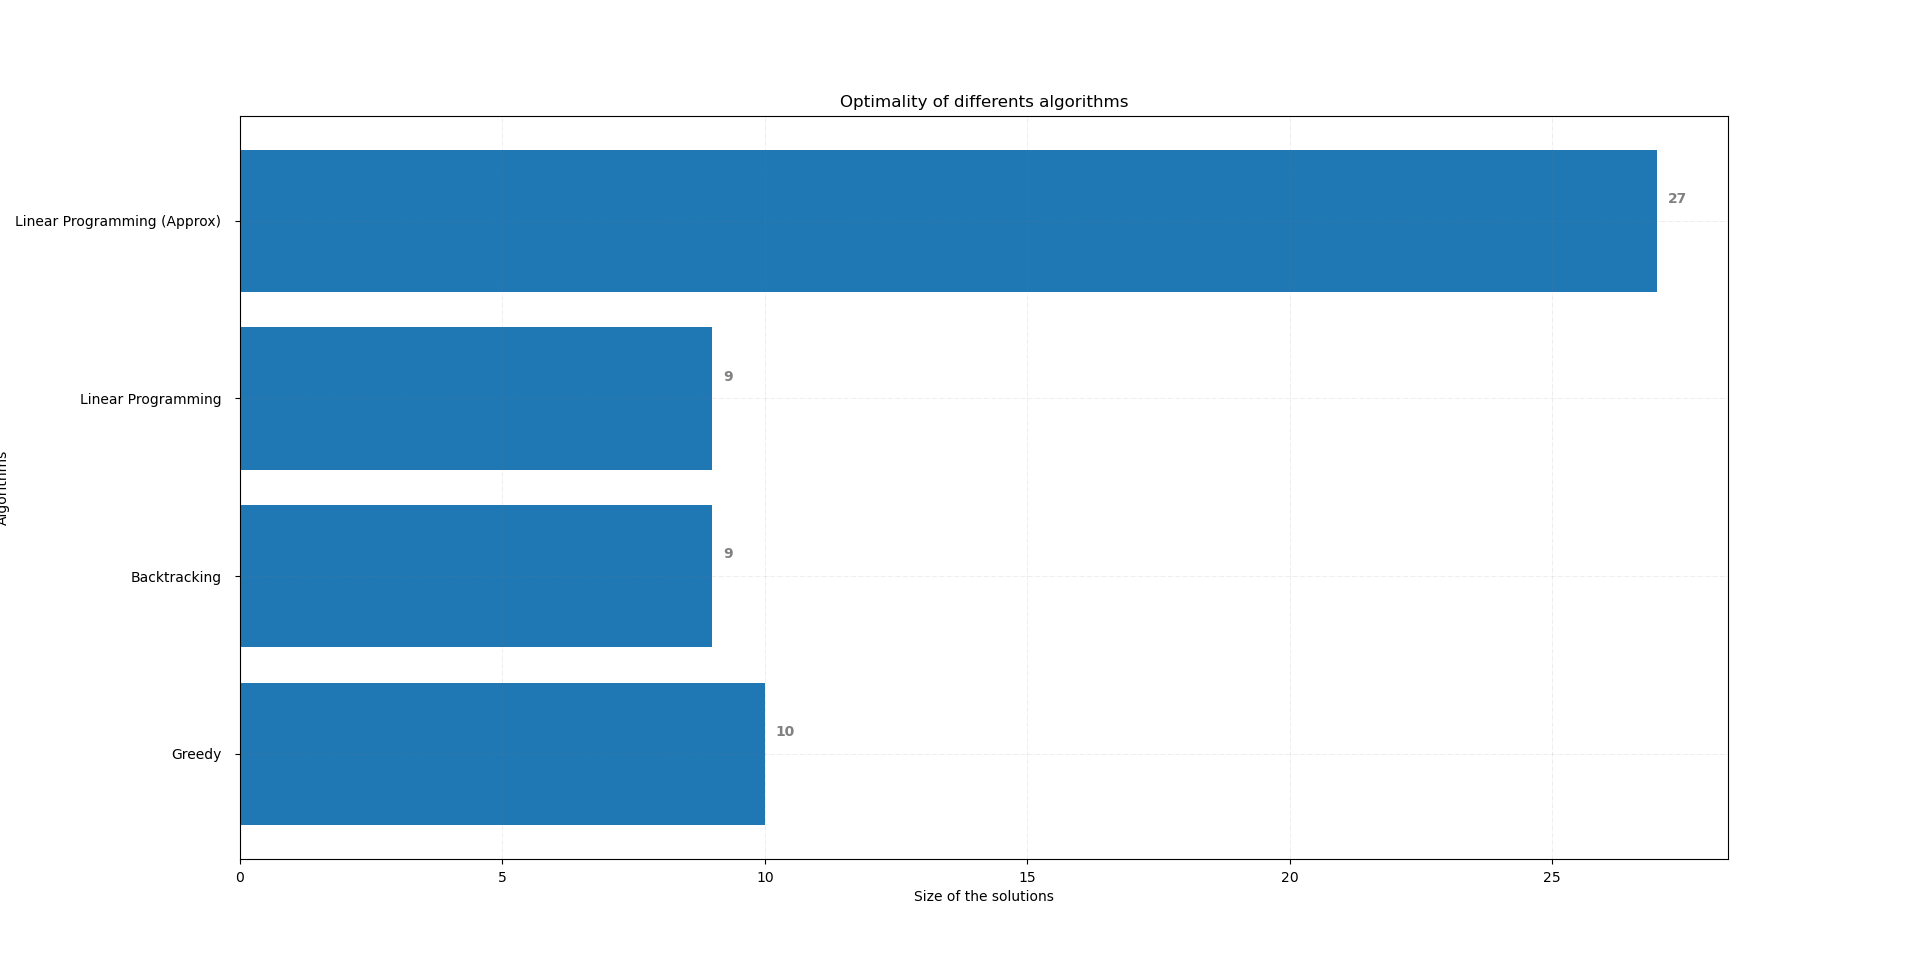
\includegraphics[width=1\textwidth]{img/comparison.png}
\end{figure}

\begin{itemize}
	\item \texttt{Our solution}: algoritmo greedy propuesto por nosotros.
	\item \texttt{As it comes}: algoritmo que analiza los rivales en el orden en el que llegan.
	\item \texttt{Sorted by Scalini ASC}: algoritmo que ordena los análisis en función de lo que tarde Scaloni en orden ascendente.
	\item \texttt{Sorted by Scalini DESC}: algoritmo que ordena los análisis en función de lo que tarde Scaloni en orden descendente.
	\item \texttt{Sorted by assistants ASC}: algoritmo que ordena los análisis en función de lo que tarden los ayudantes en orden ascendente.
\end{itemize}

Como se puede observar, el algoritmo que hace que el tiempo total requerido para que se analicen todos los rivales sea el más grande es el que ordena los análisis en función de los ayudantes de forma ascendente. Como se explicó anteriormente, esto es así porque al estar el ayudante que más vaya a tardar en el último análisis, el tiempo total de todo será el tiempo total de Scaloni en analizar los videos mas lo que vaya a tardar este último. Justamente todo lo contrario a nuestro algoritmo propuesto, que lo inserta al principio para que mientras Scaloni y el resto de ayudantes terminan de hacer sus análisis, sus tiempos se superpondran con lo que tarde el ayudante y tenga posibilidades de terminar antes que el resto de los análisis están listos.
Por otra parte, el hecho de ordenar los videos segun lo que tarde Scaloni, ya sea de forma ascendente o descendente, no implica que el tiempo total se acorte, ya que de eso depende exclusivamente los ayudantes en ver cuando se terminara el ultimo analisis y donde se sitúan los que más tarden.
Y por último, analizar los rivales tal cual llegan, es más un factor de suerte o aleatoriedad ya que el ayudante que más tarda puede ser tanto el primero como el último.
